\chapter{Resultados y discusión}

En este capítulo se presentan los resultados experimentales obtenidos mediante la simulación del
proceso evolutivo de ciclo de vida del Aedes aegypti. Los resultados obtenidos para las tasas de
desarrollo, tasas de mortalidad, dispersión y distribución de sexo son analizados con el fin de
realizar una comparación con los resultados de los estudios existentes en la literatura.

Los resultados finales, son presentados en forma de gráficos, tablas y mapas de interpolación para
una mejor comprensión de los mismos.

%~ * Introducción
\section{Descripción general del entorno de pruebas}
En esta sección se presentan las parámetros adoptados para la configuración del entorno de
pruebas, que se encuentra dividido en : características de la población inicial, periodo y datos
climatológicos, parámetros de simulador del proceso evolutivo, y por ultimo, el hardware y sistema
operativo utilizados.

\subsection{Características de la población inicial}
La cantidad de puntos de control, utilizadas para las pruebas, fue seleccionada aleatoriamente,
teniendo en cuenta que debía ser un número múltiplo de 5 ya que existen 5 tipos de zonas
(ver \secref{subsec:cap4-zonificacion}). El número seleccionado fue 25 puntos de control, de ese
modo se cuenta con 5 puntos de control por cada tipo de zona. La cantidad de larvas que
corresponden a cada punto de control se generó forma aleatoria teniendo en cuenta que los límites
establecidos para cada tipo de zona (ver \tabref{tab:cap4-puntaje-zona}). En total contabilizaron
un total de 1.146 larvas para los 25 puntos de control.

\begin{table}[!htpb]
    \begin{minipage}{\textwidth}
    \centering
        \caption{\label{tab:valores-puntos-control} Conjunto de valores de los 25 puntos de control utilizados para las pruebas.}
        \begin{tabular}{c c c c}
            \hline\\
            Identificador& Cantidad$^a$& Longitud$^b$ & Latitud$^b$\\
            \hline
            \hline \\
            198 & 40 & -57,5865364153283 & -25,3133547921686 \\
            211 & 50 & -57,5855064470667 & -25,3227427549151 \\
            209 & 10 & -57,5789833147425 & -25,3173893777233 \\
            199 & 30 & -57,5882959444416 & -25,3158764238892 \\
            201 & 36 & -57,5926303942098 & -25,3218505418179 \\
            207 & 83 & -57,5898838121785 & -25,3235961699875 \\
            200 & 35 & -57,5909137804401 & -25,3193678272972 \\
            202 & 19 & -57,5948619921102 & -25,3249926544034 \\
            210 & 55 & -57,5814724047075 & -25,3201436810523 \\
            214 & 100 & -57,5870943148027 & -25,3187471407139 \\
            215 & 60 & -57,5834894258871 & -25,3160703933853 \\
            217 & 15 & -57,5887680132287 & -25,3207255681069 \\
            218 & 5 & -57,5934887010951 & -25,3273588828944 \\
            205 & 27 & -57,5879740793598 & -25,3313154239316 \\
            206 & 30 & -57,5893902857198 & -25,3292595903167 \\
            212 & 20 & -57,5830173571008 & -25,323402212545 \\
            213 & 65 & -57,5864076692956 & -25,3267382372734 \\
            223 & 71 & -57,5754213411705 & -25,3168462682653 \\
            219 & 16 & -57,5806570131676 & -25,3155660720482 \\
            216 & 49 & -57,5829315264117 & -25,3185919685716 \\
            203 & 90 & -57,591815002669 & -25,3297250651366 \\
            204 & 67 & -57,589840896834 & -25,3332936459521 \\
            220 & 45 & -57,5908997885579 & -25,3261169237658 \\
            221 & 53 & -57,5929597250812 & -25,3234791308407 \\
            222 & 75 & -57,5874236456741 & -25,3242937494949 \\
        \end{tabular}
        \footnotetext[1]{Cantidad de larvas correspondientes al punto de control.}
        \footnotetext[2]{Coordenadas geográficas correspondientes al punto de control.}
    \end{minipage}
\end{table}

En la \tabref{tab:valores-puntos-control}, se pueden apreciar los valores de los 25 puntos de
control utilizados. La distribución geográfica se realizó de forma aleatoria y no uniforme
en un área de total de $3,028 km^{2}$, que corresponde al área resultante de la unión de 2
barrios, Terminal e Hipódromo, de la ciudad de Asunción (\figref{fig:distribucion-puntos}).
Es importante aclarar que la selección de los barrios solo tiene relevancia, en la simulación,
para la obtención de datos climatológicos correspondientes para dicha región.

\begin{figure}[!htpb]
\centering
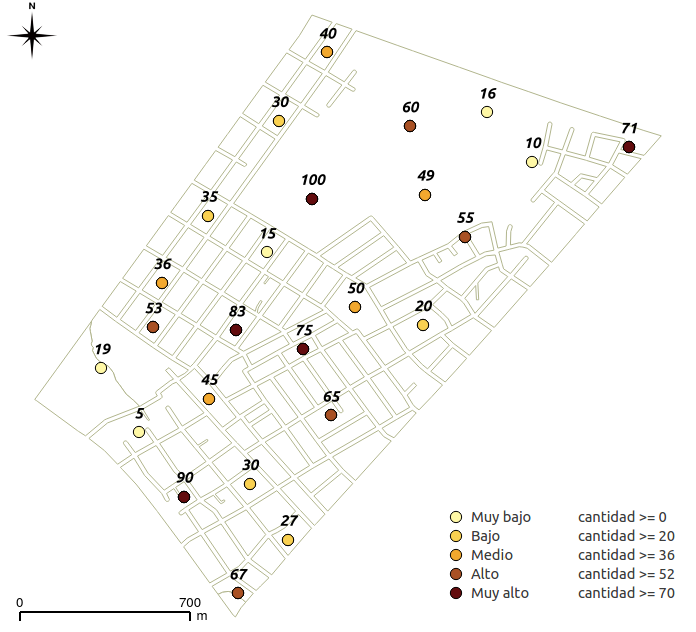
\includegraphics[width=0.9\textwidth]{./capitulo-6/graphics/extension-poblacion.png}
\caption{\label{fig:distribucion-puntos}Distribución geográfica de los 25 puntos de control.}
\end{figure}


\subsection{Periodo y datos climatológicos}
La mayoría de los estudios, que posteriormente fueron utilizados para las comparaciones, se basan
en someter a un grupo de individuos por un periodo de tiempo fijo utilizando una temperatura
constante. El mayor periodo observado fue de $46,83$ días en \cite{rueda1990temperature}, motivo
por el cual el tamaño del periodo fue establecido en 50 días.

En total se realizaron 10 iteraciones de 50 días cada una con las siguientes temperaturas :
15\textcelsius , 18\textcelsius , 20\textcelsius , 22\textcelsius , 24\textcelsius , 25\textcelsius
, 26\textcelsius , 27\textcelsius , 30\textcelsius , 34\textcelsius. De este modo se pueden simular
el proceso evolutivo de los individuos de la población a 10 temperaturas constantes.

\begin{figure}[!htpb]
\centering
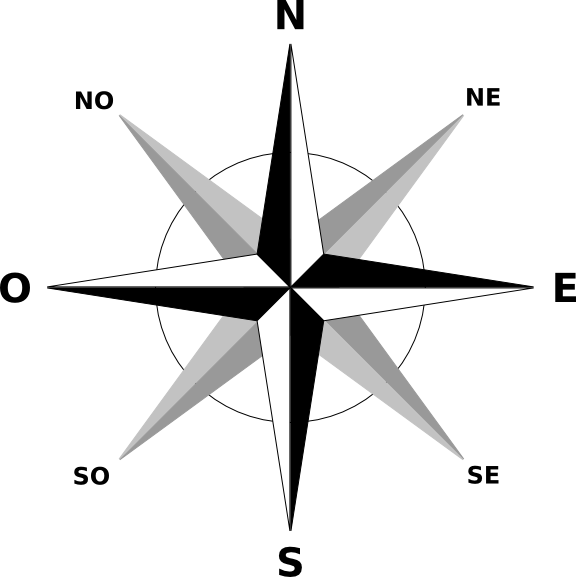
\includegraphics[width=0.5\textwidth]{./capitulo-6/graphics/rosa-de-vientos.png}
\caption{\label{fig:puntos-cardinales}Representación de los puntos cardinales.}
\end{figure}

La dirección al igual que la temperatura fue establecida como una constante para las pruebas, para
facilitar el análisis de la dispersión de los focos. La dirección del viento seleccionada fue la
suroeste (\figref{fig:puntos-cardinales}), que genera un ángulo que varía entre $202,5^{\circ}$ a
$247,5^{\circ}$.

\subsection{Parámetros de simulador del proceso evolutivo}
Los parámetros del simulador del proceso evolutivo, en su mayoría son calculados con datos
biológicos correspondientes al área de estudio. Obtener dichos datos requieren minuciosos estudios
de campo que escapan del alcance de este trabajo. Finalmente se optó por utilizar configuraciones
provenientes del material bibliográfico disponible que utilizado para el diseño y desarrollo del
modelo encargado de realizar la simulación de la ecología del vector.

El tamaño del radio, $r$, fue configurado en $200$ metros, para el cálculo de la densidad relativa
de larvas, $u(x,y)$ (ver \secref{subsec:cap4-zonificacion}). De este modo se incluirán todos los
puntos de control que se encuentren en un área de $125,663 \times 10^{3}$ $m^{2}$.

En cuanto a los sitios de reproducción, los parámetros $bs_{min}$ y $bs_{max}$ fueron tomados
configurados según lo observado en \cite{otero2006stochastic, otero2008stochastic}, siendo $15$ y
$50$ los valores adoptados respectivamente.  El valor de $bs_{med}$ fue establecido, en $32,5$,
realizando un promedio entre $bs_{min}$ y $bs_{max}$.

En la \tabref{tab:coef-sharpe-demichele}, se pueden apreciar los coeficientes para el modelo
simplificado de Sharpe y DeMichele, con inhibición de altas temperaturas de Schoolfield (ver
\secref{subsec:cap4-tasas de desarrollo}) utilizados para calcular las tasas de desarrollo media
en $dias^{-1}$ fueron tomados de : \cite{rueda1990temperature} para el desarrollo larvario y el
desarrollo pupal, y de \cite{otero2006stochastic} para la eclosión de huevos, ciclo gonotrófico para hembras nulíperas y paridas.

\begin{table}[!htpb]
\begin{minipage}{\textwidth}
    \centering
    \caption{ \label{tab:coef-sharpe-demichele} Coeficientes para el modelo simplificado de Sharpe y DeMichele, con inhibición de altas temperaturas presentado por Schoolfield.}
    \begin{tabular}{p{6cm} c r r r r }
        \hline \\
        Ciclo de desarrollo    & $R(298K)$ & $\Delta H_{A}$ & $\Delta H_{H}$ & $\Delta T_{1/2}$  \\
        \hline
        \hline\\
        Eclosión de los huevos$^a$ & 0,24000 & 10798,00 &  100000,00  & 14184,000\\
        Desarrollo larvario$^b$    & 0,20429 & 36072,78 &   59147,51  &   301,560\\
        Desarrollo pupal$^b$       & 0,74423 & 19246,42 &    5954,35  &   302,687\\
        Ciclo gonotrófico (AN)$^c$ & 0,21600 & 15725,00 & 1756481,00  &   447,200\\
        Ciclo gonotrófico (AP)$^c$ & 0,37200 & 15725,00 & 1756481,00  &   447,200\\
    \end{tabular}
    \footnotetext[1]{Coeficientes tomados \cite{otero2006stochastic}.}
    \footnotetext[2]{Coeficientes tomados \cite{rueda1990temperature}.}
    \footnotetext[3]{Coeficientes, para el desarrollo del ciclo gonotrófico de hembras paridas (AP) y nulíparas (AN), tomados \cite{otero2006stochastic}.}
\end{minipage}
\end{table}

Las configuraciones adoptadas de
\cite{otero2006stochastic,otero2008stochastic,rueda1990temperature}, resultan válidas para las
pruebas, sin embargo pueden requerir una revisión general con el fin de realizar los ajustes
correspondientes teniendo en cuenta los datos ecológicos del área de estudio.

\subsection{Hardware y sistema operativo utilizados}
El hardware y el sistema operativo utilizados para realizar las pruebas, tienen las siguientes
características :
\begin{itemize}
\item Procesador : Intel Core i5-2430M
\item CPU : 2.40GHz × 4
\item Memoria : 8 GB
\item Sistema operativo : Ubuntu 13.10 x 64
\end{itemize}


\subsection{Tasa de desarollo}
Verificar las tasas de desarrollo de los individuos de la población de forma a validar
si el incremento de la madurez del individuo es correcta. Se debe contar con el tiempo
promedio de de la duración de cada estado, en días, para compararlos con los promedios
generales.

\begin{itemize}
    \item Temperatura constante
    \item Duración en promedio en cada estado a temperatura constante
    \item Desviación estándar
    \item Calcular el error
\end{itemize}

\section{Ciclo gonotrófico}
Para el análisis de la tasa de desarrollo, en días, del ciclo gonotrófico de las hembras del Aedes
aegypti, se clasificó la población en hembras núliparas y paridas. En la
\tabref{tab:ciclo-gonotrofico-test} se puede observar una media de $5,03$ días para las hembras
nulíparas y  $2,92$ días para las paridas para una temperatura aproximada de $25,11$ \textcelsius.

\begin{table}[!htbp]
    \begin{minipage}{\textwidth}
        \centering
        \caption{ \label{tab:ciclo-gonotrofico-test} Análisis de duración del ciclo gonotrófico
        de la hembra de Aedes aegypti nueve temperaturas constantes  (18-34 \textcelsius).}
        \begin{tabular}{l *{10}{c} }
            \hline \\
            & &  & &  & &  &  &  &  & Media\\
            Población & 18\textcelsius & 20 \textcelsius & 22 \textcelsius & 24 \textcelsius
                      & 25 \textcelsius & 26\textcelsius  & 27 \textcelsius & 30 \textcelsius
                      & 34\textcelsius & General\\

            \hline
            \hline \\
            Nulíparas\footnote{Hembras nulíparas que no han ovipuesto.}
                        & 8,97 & 7,4  & 6,13  & 5,08  & 4,63 & 4,22  & 3,85 & 2,94 & 2,06 & 5,03\\
            Paridas\footnote{Hembras que ya han realizado al menos una ovipostura.}
                        & 5,21 & 4,3  & 3,56  & 2,95  & 2,69 & 2,45  & 2,24 & 1,71 & 1,2 & 2,92\\
            Media \footnote{Promedio general de la duración general del ciclo gonotrófico para las
            hembras}
                        & 7,09 & 5,85 & 4,85  & 4,02  & 3,66 & 3,34  & 3,05 & 2,33 & 1,63 & 3,98\\
        \end{tabular}
    \end{minipage}
\end{table}

Las variaciones en la temperatura influyen en tiempo de digestión de la sangre y el
desarrollo de los ovarios, a medida que la temperatura desciende, la digestión y por ende el ciclo
gonotrófico tomará más tiempo (\figref{fig:ciclo-gonotrofico-temperatura}). En \cite{edman1987host}
se observó que hembras nulíparas de Aedes aegypti poseen un proceso de digestión es más lento en
las hembras paridas y por ende el ciclo gonotrófico de las mismas tiene a ser más largo. Existen
diversos estudios, que han reportado que el patrón diario de alimentación de los mosquitos, varia
de acuerdo a las localidades y subespecies. A continuación se mencionaran algunos estudios
realizados correspondientes a la duración del ciclo gonotrófico, con el fin de realizar una
comparación con los resultados obtenidos mediante el proceso evolutivo.

\begin{figure}[!htbp]
    \centering
    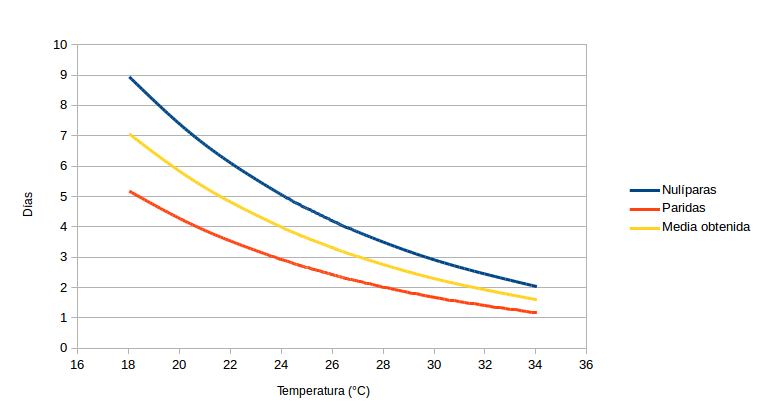
\includegraphics[width=1\textwidth]{capitulo-6/graphics/ciclo-gonotrofico-temperatura.png}
    \caption{\label{fig:ciclo-gonotrofico-temperatura} Tasa de desarrollo, en días, del ciclo
    gonotrófico de hembras nulíparas, hembras paridas y la media general a nueve temperaturas
    constantes (18-34 \textcelsius).}
\end{figure}

En \cite{beltran2001bionomia} se determinó que la duración del ciclo gonotrófico del Aedes
aegypti, para los siguientes municipios de México en, 3 días para Tamazula de Gordiano a una
temperatura de $21,5$ \textcelsius, 3 días para Techaluta de Montenegro a $22,8$ \textcelsius, 4
días para Tuxpan a 22 \textcelsius y 5 días para CD Zacoalco de Torres a $22,7$ \textcelsius.

En \cite{luevano1993ciclo}, el autor determinó la duración del ciclo gonotrófico de las
poblaciones naturales de Aedes aegypti en el área metropolitana de Monterrey, Nuevo León. México,
en cinco días, a una temperatura promedio de $25,5$ \textcelsius.

En \cite{trpis1986dispersal} los autores reportaron una duración del ciclo gonotrófico en Kenia a
nivel rural de, 5 a 7 días para el primer ciclo (hembras nulíparas) y de 4 a 5 días para los
siguientes ciclos (hembras paridas). El método utilizado fue de captura con cebo humano de
mosquitos de Aedes aegypti.

Según \cite{sivanathan2006ecology} el ciclo gonotrófico del aAedes aegypti y Aedes albopictus se
encuentra acotada entre $2,73$ a 3 días respectivamente.

Las diferentes condiciones climáticas y la capacidad de adaptación en habitad específicos, del
Aedes aegypti, son las responsables de diferencias que se puedan tener entre cepas del mosquito.
La duración del ciclo gonotrófico obtenida, depende de los coeficientes para el modelo de
maduración enzimática de \cite{sharpe1977reaction} que fue tomado de \cite{otero2006stochastic},
que según los autores fue tomado de \cite{focks1993dynamic}.


\section{Vuelo y dispersión}
Para el análisis de la distancia recorrida, en metros, del adulto de Aedes aegypti, se realizaron
pruebas a 9 temperaturas constantes (15-34\textcelsius), solo las hembras que han ovipuesto al
menos una vez fueron incluidas. En la tabla \ref{tab:pomedio-vuelo-test} se presentan los
resultados obtenidos para la disperción de las hembras adultas del aedes aegypit agrupadas por el
tipo su tipo de zona, en general se obtuvo un promedio de $65,74$, $63,97$ $1308,19$ metros para las zonas buena, normal y malas respectivamente. Existen diversos estudios, que han reportado que
la disperción del aedes aegypti en relación a las caracteristicas de su ambiente. A continuación
se mencionaran algunos estudios realizados, con el fin de realizar una comparación con los resultados obtenidos.

En \cite{cabezas2005dengue} señalan que por lo general mosquito no sobrepasa los 50 a 100 metros
durante su vida, ya que tiende a permanecer en el lugar donde emergió.

Según \cite{ThironIzcazaJ2003} por lo general, la hembra de Ae. aegypti, permanece físicamente en
donde emergió, siempre y cuando no halla algún factor que la perturbe o no disponga de huéspedes,
sitios de reposo y de postura. En caso de no haber recipientes adecuados, la hembra grávida es capaz de volar hasta tres kilómetros en busca de este sitio.

Los autores de \cite{dengueUruguayCap8} señalan que, para las estrategias de control de Aedes
aegypti en zonas urbanas donde existen brotes de dengue y fiebre amarilla se asume que los
mosquitos tienen un rango de vuelo durante su vida de 50 a 100 metros.

En \cite{luevano1993ciclo} se reporta, que el aedes aegypti es un mosquito doméstico que
generalmente esta confinado a las casas donde se cria, tiene un rango de vuelo corto, entre 23 a 50 metros, y raramente se dispersa a largas distancias.

\cite{mcdonald1977population} en Kenia, liberó poblaciones de Aedes aegypti a las distancias de,
200, 400 y 800 metros, y observó que aproximadamente el 50 \% de los mosquitos marcados se
dispersaron a 200 metros del punto en el cual fueron liberados, un 10 \% a 400 metros y solamente
el 1 \% se dispersó a 800 metros.

En \cite{trpis1986dispersal}, los autores reportaron que en Kenia, que la tasa media de dispersión
de las hembras fue de 57 metros. La distancia máxima de las hembras durante 24 horas fue de 154
metros.

La mayoría de los estudios coinciden que, los adultos del aedes aegypti, en condiciones óptimas de
disponibilidad de alimento y sitios adecuados de ovipostura, tienden a permanecer en el lugar
donde emergieron, con una dispersión media estimada entre 50 y a 100 metros, su presencia es
prácticamente un indicio certero de la proximidad de los criaderos. En caso de no contar con
sitios adecuados de ovipostura y disponibilidad de alimento tienden a dispersarme una mayor
distancia en busca de mejores condiciones.

\begin{table}
    \begin{minipage}{\textwidth}
        \caption{ \label{tab:pomedio-vuelo-test} Análisis de la dispersión, por zona, del adulto
        de Aedes aegypti diez temperaturas constantes (15-34 \textcelsius).}
        \begin{tabular}{p{4cm} *{4}{c}  }
          \hline \\
          Temperatura (\textcelsius)& Buena & Normal & Mala & Media Obtenida\\
          \hline
          \hline \\
          18 & 89,06 & 66,61 & 1274,97 & 476,88\\
          20 & 66,52 & 73,53 & 1516,43 & 552,16\\
          22 & 77,89 & 63,78 & 1003,9 & 381,86\\
          24 & 60,28 & 62,31 & 1077,6 & 400,06\\
          25 & 54,52 & 63,66 & 1397,31 & 505,16\\
          26 & 61,61 & 60,79 & 1509,67 & 544,02\\
          27 & 65,24 & 63,72 & 1433,58 & 520,85\\
          30 & 62,61 & 59,56 & 1213,1 & 445,09\\
          34 & 53,92 & 61,75 & 1347,13 & 487,6\\
          Media General & 65,74 & 63,97 & 1308,19 & 479,3\\
        \end{tabular}
    \end{minipage}
\end{table}

\section{Distribución de Sexo}
Se realizó un análisis para determinar la distribución del sexo del Aedes aegypti. Según
\cite{otero2006stochastic}, alrededor de la mitad de los adultos emergentes son hembras, y se
define una proporción de 1.02:1 macho: hembra. Los autores de \cite{manrique1998desarrollo} la
proporción sexual promedio de adultos emergidos es de $3$ machos por $2,75$ hembras, lo cual no representa una diferencia significativa de una relación 1:1 en las proporciones sexuales.

En general se realizaron pruebas variando la cantidad de individuos de la población, los
resultados se pueden apreciar en la tabla \tabref{tab:distribucion-sexo-test}, donde se observa que
existe una relación 1:1 para la distribución del sexo de los mosquitos.

\begin{table}
    \centering
        \caption{ \label{tab:distribucion-sexo-test} Análisis de la distribución del sexo de Aedes
        aegypti.}
        \begin{tabular}{l c c c }
            \hline \\
            Total de & Adultos & Adultos & Relación \\
            adultos  & machos  & hembras & (macho:hembra) \\
            \hline
            \hline \\
            912    &  461    &  451    &  0,99 : 1,01 \\
            1581   &  812    &  769    &  0,97 : 1,03 \\
            4154   &  2084   &  2070   &  1    : 1 \\
            9722   &  4940   &  4782   &  0,98 : 1,02 \\
            9045   &  4472   &  4573   &  1,01 : 0,99 \\
            16248  &  8104   &  8144   &  1    : 1 \\
            30693  &  15418  &  15275  &  1    : 1 \\
            28411  &  14224  &  14187  &  1    : 1 \\
        \end{tabular}
\end{table}

\section {Análisis espacial de los resultados}

Los datos obtenidos mediante el simulador del proceso evolutivo, contienen información que nos
permiten analizarlos en el contexto de un SIG, para identificar los focos de infestación mediante
técnicas de interpolación espacial.

Los niveles de riesgos fueron determinados de acuerdo a los tipos de zonas determinados en la
\secref{subsec:cap4-zonificacion}. Se consideran de mayor riesgo las zonas propicias para el
desarrollo del Aedes aegypti. En la \tabref{tab:niveles-riesgo-zonas}, se presentan los niveles de
riesgo definidos según la \tabref{tab:cap4-puntaje-zona}.


\begin{table}[!hptb]
    \begin{minipage}{\textwidth}
\begin{center}
    \caption{\label{tab:niveles-riesgo-zonas} Niveles de infestación de las zonas.}
    \begin{tabular}{p{3cm} l c c c}
        \hline \\
         Niveles de  & Color & Mínimo$^a$ & Máximo$^a$ \\
         infestación & identificador & $u(x,y)$   & $u(x,y)$  \\
        \hline
        \hline\\
        Muy bajo  & \cellcolor{muybajo}& 0  & 19 \\
        Bajo    & \cellcolor{bajo}& 20 & 35 \\
        Normal & \cellcolor{normal}& 36 & 51 \\
        Alto   & \cellcolor{alto}& 52 & 69 \\
        Muy Alto & \cellcolor{muyalto} & 70 & --$^b$\\
    \end{tabular}
    \footnotetext[1]{Rango mínimo y máximo de $u(x,y)$ permitido para el tipo de zona.}
    \footnotetext[2]{No se estableció un límite superior para este nivel. }
\end{center}
    \end{minipage}
\end{table}

\subsection{Análisis general de la población}
La distribución geográfica, dispersión y niveles de infestación de las poblaciones de Aedes aegypti
son presentadas como mapas de interpolación, donde para la interpolación espacial fueron
seleccionados los individuos pertenecientes a las poblaciones correspondientes a un día del
periodo de simulación. Para el análisis espacial fueron seleccionadas los datos obtenidos mediante
la simulación del proceso evolutivo a 6 temperaturas constantes(15 a 34 \textcelsius). Los días
del periodo de simulación, utilizados para generar los mapas de interpolación, fueron
seleccionados teniendo en cuenta el crecimiento y decrecimiento de la población observado en
la \figref{fig:desarrollo-poblacion-all} con el fin de resaltar los eventos más relevantes de cada
población.

\begin{figure}[!htbp]
    \centering
    \begin{subfigure}[b]{0.45\textwidth}
            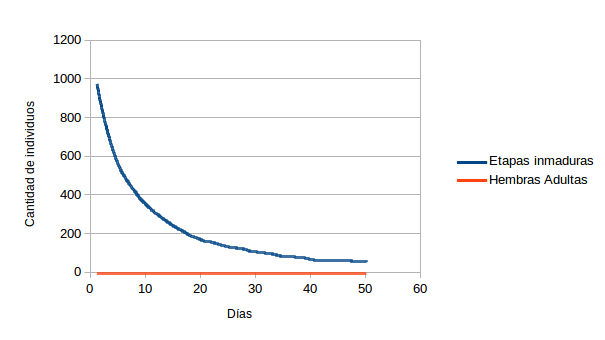
\includegraphics[width=\textwidth]{capitulo-6/graphics/desarrollo-poblacion-15.png}
            \caption{\label{fig:desarrollo-poblacion-15}Población a 15 \textcelsius.}
    \end{subfigure}
    ~~~~
    \begin{subfigure}[b]{0.45\textwidth}
            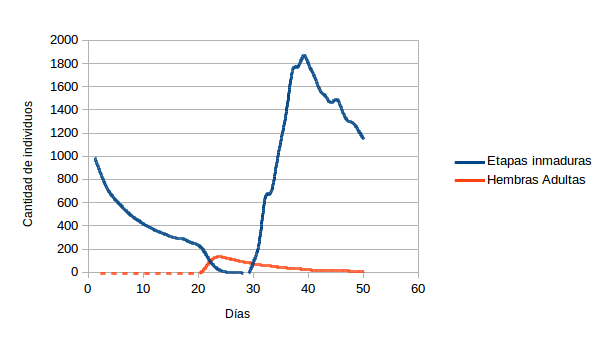
\includegraphics[width=\textwidth]{capitulo-6/graphics/desarrollo-poblacion-20.png}
            \caption{\label{fig:desarrollo-poblacion-20}Población a 20 \textcelsius.}
    \end{subfigure}

    \begin{subfigure}[b]{0.45\textwidth}
            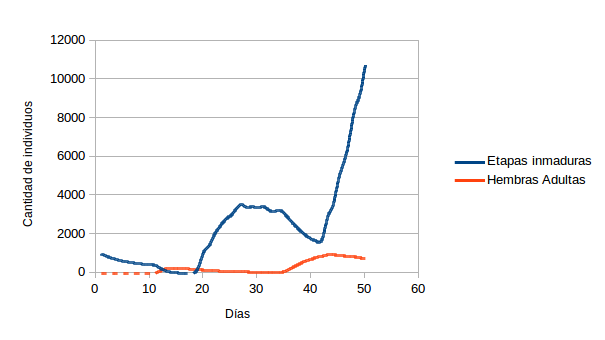
\includegraphics[width=\textwidth]{capitulo-6/graphics/desarrollo-poblacion-24.png}
            \caption{\label{fig:desarrollo-poblacion-24}Población a 24 \textcelsius.}
    \end{subfigure}
    ~~~~
    \begin{subfigure}[b]{0.45\textwidth}
            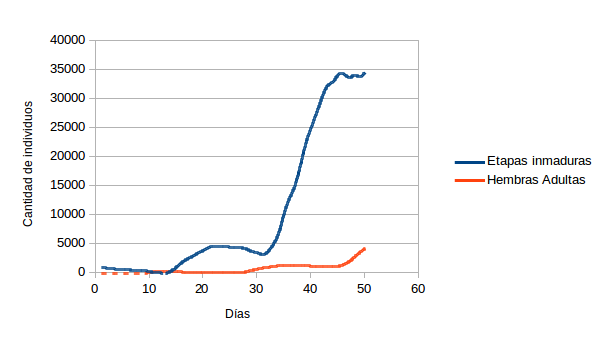
\includegraphics[width=\textwidth]{capitulo-6/graphics/desarrollo-poblacion-27.png}
            \caption{\label{fig:desarrollo-poblacion-27}Población a 27 \textcelsius.}
    \end{subfigure}

    \begin{subfigure}[b]{0.45\textwidth}
            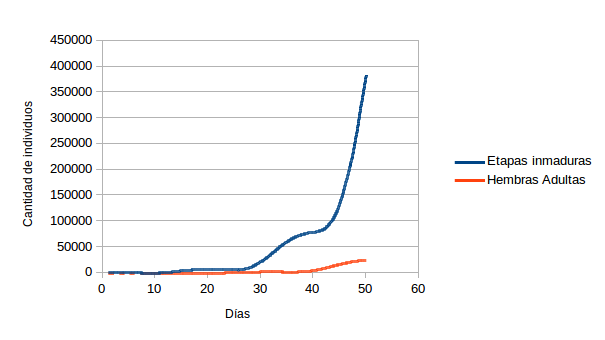
\includegraphics[width=\textwidth]{capitulo-6/graphics/desarrollo-poblacion-30.png}
            \caption{\label{fig:desarrollo-poblacion-30}Población a 30 \textcelsius.}
    \end{subfigure}
    ~~~~
    \begin{subfigure}[b]{0.45\textwidth}
            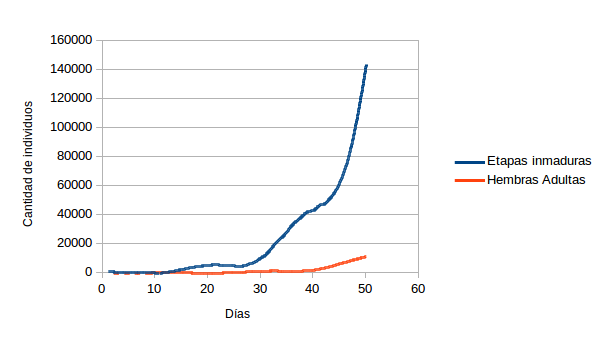
\includegraphics[width=\textwidth]{capitulo-6/graphics/desarrollo-poblacion-34.png}
            \caption{\label{fig:desarrollo-poblacion-34}Población a 34 \textcelsius.}
    \end{subfigure}

    \caption{\label{fig:desarrollo-poblacion-all} Análisis del comportamiento de la población de mosquitos en relación al tiempo a 6 temperaturas constantes (15-34 \textcelsius).}
\end{figure}

En la \figref{fig:desarrollo-poblacion-all}, se pueden observar el comportamiento de las
poblaciones a 6 temperaturas constantes (15-34 \textcelsius). En general, para todos los casos, la
población inicial sufre un decrecimiento causada por la mortalidad diaria de los individuos a
temperaturas entre 15 y 34 \textcelsius, y por la emergencia de adultos a temperaturas entre 20 y
34 \textcelsius. La aparición de adultos implica que la población de individuos en etapas
inmaduras (huevos, larvas y pupas), llegaron a completar su ciclo de desarrollo para dar lugar a
mosquitos adultos, por lo tanto la población de individuos en etapas inmaduras tiende a disminuir
y mientras que la población de mosquitos adultos tiende a aumentar. El crecimiento de la población
se debe a que las hembras adultas pertenecientes a la población de mosquitos, culminaron su ciclo
gonotrófico y dieron lugar la ovipostura.

En la \secref{sec:tasas-desarrollo-mortalidad} se presentaron las tasas de desarrollo obtenidas a
diferentes temperaturas, en donde se pudo observar que a medida que la temperatura aumenta, las
tasas de desarrollo son menores, motivo por el cual las poblaciones de individuos en etapas
inmaduras, sometidos a temperaturas más elevadas, tienden a disminuir su tamaño rápidamente debido
a que se desarrollan con mayor rapidez, dando lugar a su etapa de adulto. Del mismo modo el ciclo
gonotrófico, presentado en la \secref{sec:tasa-ciclo-gonotrofico}, para las hembras adultas
tienden a disminuir su duración, causando que el intervalo entre oviposturas disminuya, en
consecuencia el tamaño de la población de individuos en etapas inmaduras aumenta rápidamente.

Todas las poblaciones, sometidas a temperaturas que permitieron la aparición de adultos,
experimentaron una dispersión hacia el noreste debido a que la dirección del viento utilizada era
de sureste.
%Tendencia de dispersión causada porque la dirección del viento es suroeste

%Solo las hembras adultas se muestran que representa el 50\% de la población

\subsection{Análisis de la población a 15 \textcelsius}
%Población a 15 C
En la \figref{fig:desarrollo-poblacion-15}, se puede apreciar que el tamaño de la población a 15
\textcelsius, tiende a disminuir con el transcurrir del tiempo. Considerando que el estado inicial
de los individuos, para la simulación del proceso evolutivo, es el de larva, tenemos una tasa de
desarrollo igual a $44,33$ días de desarrollo
(\tabref{tab:desarrollo-larva-rueda1990temperature-test}), para las larvas.

\begin{figure}[!htbp]
    \centering
    \begin{subfigure}[b]{0.45\textwidth}
            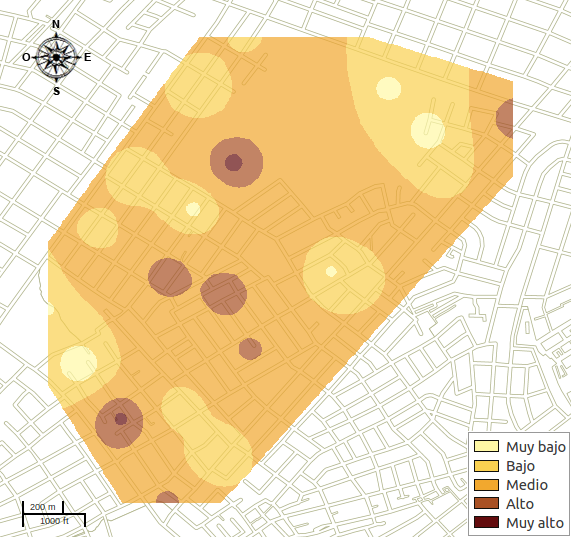
\includegraphics[width=\textwidth]{capitulo-6/graphics/raster/temp-15-0.png}
            \caption{\label{fig:niveles-infestacion-15-a}Primer día de simulación.}
    \end{subfigure}
    ~~
    \begin{subfigure}[b]{0.45\textwidth}
            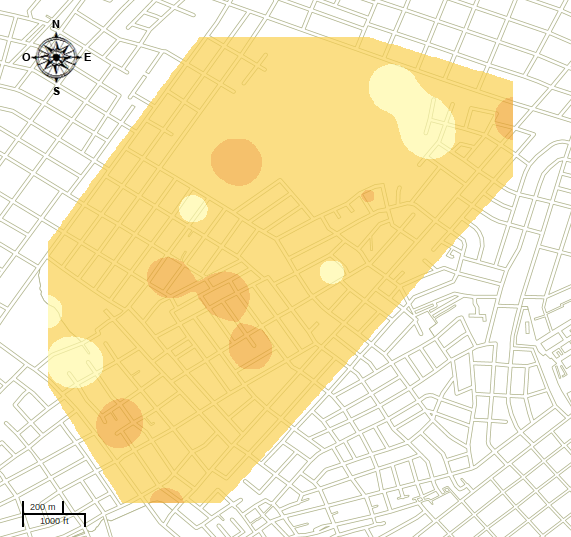
\includegraphics[width=\textwidth]{capitulo-6/graphics/raster/temp-15-2.png}
            \caption{\label{fig:niveles-infestacion-15-b}Día número 3 de simulación.}
    \end{subfigure}
    \begin{subfigure}[b]{0.45\textwidth}
            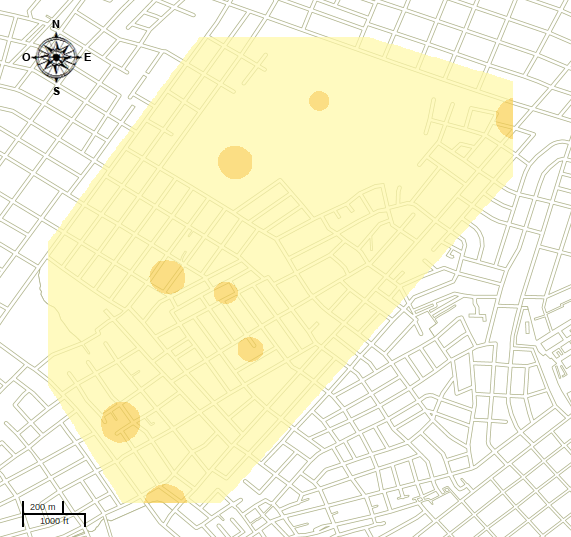
\includegraphics[width=\textwidth]{capitulo-6/graphics/raster/temp-15-7.png}
            \caption{\label{fig:niveles-infestacion-15-c}Día número 8 de simulación.}
    \end{subfigure}
    ~~
    \begin{subfigure}[b]{0.45\textwidth}
            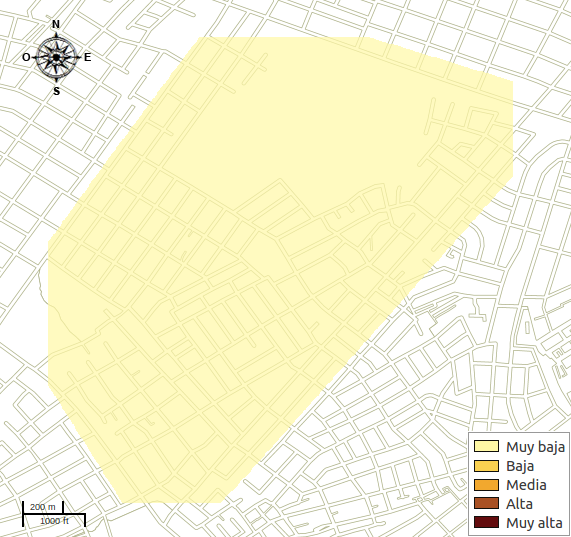
\includegraphics[width=\textwidth]{capitulo-6/graphics/raster/temp-15-9.png}
            \caption{\label{fig:niveles-infestacion-15-d}Día número 10 de simulación.}
    \end{subfigure}
    \caption{\label{fig:niveles-infestacion-15} Mapas de interpolación de la población correspondientes a los días 1, 3, 8 y 10 de simulación a 15 \textcelsius.}
\end{figure}

En un periodo de 50 días a 15 \textcelsius, no se pueden observar mosquitos adultos motivo por el
cual la población tiende a disminuir su tamaño y por ende el riesgo de infestación del área de
estudio. En la \figref{fig:niveles-infestacion-15} se puede observar el rápido decrecimiento de la
población y de los niveles de infestación. Para el octavo día, en la
\figref{fig:niveles-infestacion-15-c}, se puede apreciar el rápido decrecimiento en los niveles de
infestación, debido a la disminución de la población observados en
\figref{fig:desarrollo-poblacion-15}. A partir del décimo día,
\figref{fig:niveles-infestacion-15-d}, los niveles de infestación se mantienen constantemente
bajos, por lo que los mapas de interpolación se mantienen constantes hasta el final del periodo de
simulación.

Debido a que no se pudieron observar adultos la población inicial no sufrió ninguna dispersión, ya
que las etapas inmaduras del mosquito son etapas acuáticas.

\subsection{Análisis de la población a 20\textcelsius}
%Población a 20 C
En la \figref{fig:desarrollo-poblacion-20}, se puede observar el comportamiento de la población a
20 \textcelsius, en donde la población de individuos en sus etapas inmaduras va decreciendo hasta
desaparecer temporalmente el día 28, no así la población de adultos. En la
\figref{fig:niveles-infestacion-20-b}, se puede observar que no existen mosquitos en sus etapas
inmaduras, para generar un mapa de interpolación del área, sin embargo se pueden observar la
distribución geográfica de las hembras adultas. Desde el día 21, en la
\figref{fig:desarrollo-poblacion-20}, comienzan a observarse los primeros mosquitos adultos, que a
partir del día 30, las hembras adultas, comienzan oviponer, generando la reaparición de la
población de mosquitos que alcanza su máximo valor en el día 39.

\begin{figure}[!htbp]
    \centering
    \begin{subfigure}[b]{0.45\textwidth}
            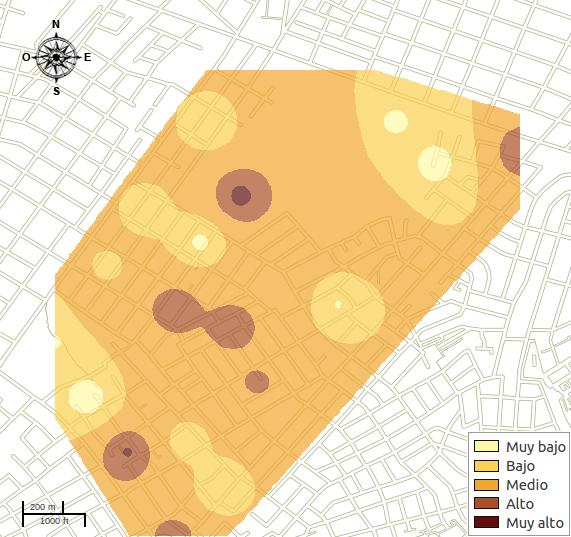
\includegraphics[width=\textwidth]{capitulo-6/graphics/raster/temp-20-0.png}
            \caption{\label{fig:niveles-infestacion-20-a}Primer día de simulación.}
    \end{subfigure}
    ~~
    \begin{subfigure}[b]{0.45\textwidth}
            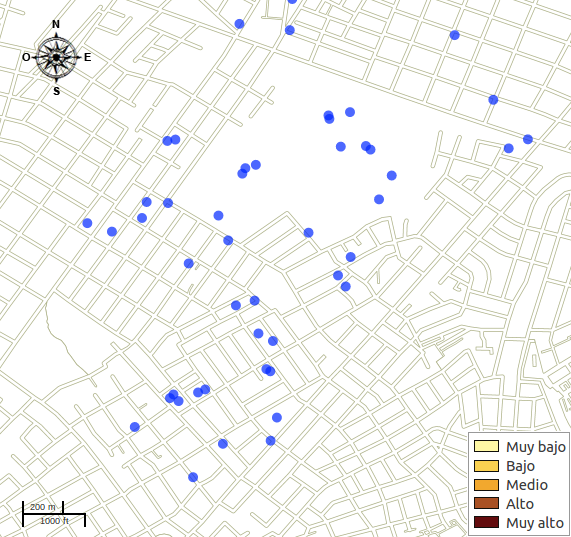
\includegraphics[width=\textwidth]{capitulo-6/graphics/raster/temp-20-28.png}
            \caption{\label{fig:niveles-infestacion-20-b}Día número 28 de simulación.}
    \end{subfigure}

    \begin{subfigure}[b]{0.45\textwidth}
            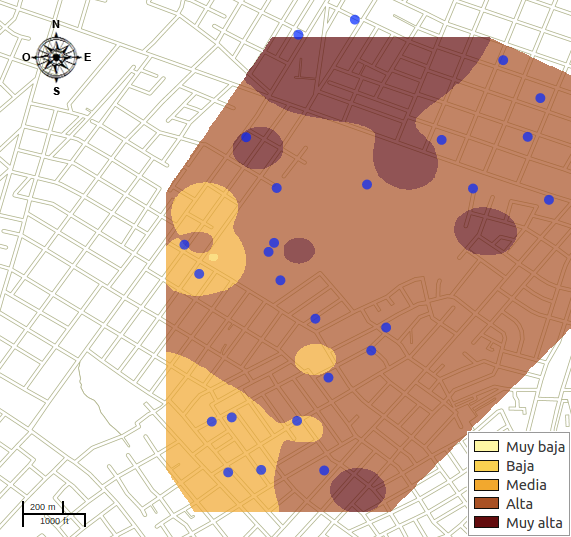
\includegraphics[width=\textwidth]{capitulo-6/graphics/raster/temp-20-35.png}
            \caption{\label{fig:niveles-infestacion-20-c}Día número 36 de simulación.}
    \end{subfigure}
    ~~
    \begin{subfigure}[b]{0.45\textwidth}
            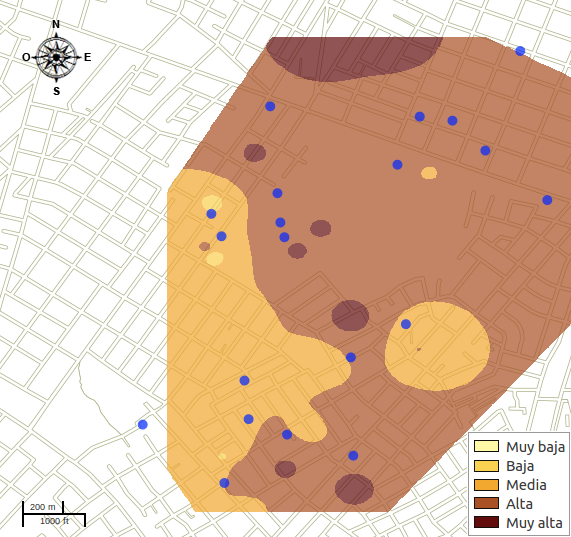
\includegraphics[width=\textwidth]{capitulo-6/graphics/raster/temp-20-38.png}
            \caption{\label{fig:niveles-infestacion-20-d}Día número 39 de simulación.}
    \end{subfigure}

    \caption{\label{fig:niveles-infestacion-20} Mapas de interpolación de la población correspondientes a los días 1, 29, 36 y 39 de simulación a 20 \textcelsius, y la distribución de las hembras adultas (puntos en azul). }
\end{figure}

En la \figref{fig:niveles-infestacion-20} se puede apreciar los niveles de infestación para los
días 1, 28, 36 y 38 del periodo de simulación. Además se observa el desplazamiento de los focos de
infestación, causado por la dispersión de los adultos, que pasan de su estado inicial
(\figref{fig:niveles-infestacion-20-a}), a generar nuevos focos
(\figref{fig:niveles-infestacion-20-c} y \figref{fig:niveles-infestacion-20-d}). Cabe resaltar
que, un aumento en el tamaño de la población no necesariamente implica mayores niveles de
infestación. Esto se puede observar realizando una comparación entre los niveles de infestación
presentados en las \figref{fig:niveles-infestacion-20-c} y \figref{fig:niveles-infestacion-20-d},
y el tamaño de la población para los días 36 y 39 del periodo de simulación, en donde el día 39
cuenta con una población de mayor tamaño que el día 36, pero en este último se observan mayores
niveles de infestación. Esto se debe a que los mapas de interpolación dependen de la distribución
geográfica de los individuos de la población y la concentración de los mismos en $(x,y)$.

A 20 \textcelsius se observa el desplazamiento de los focos de infestación en dirección al
noreste, debido a que la dirección del viento utilizada es igual al sureste y los mosquitos
adultos tienden a volar en dirección contraria al viento. Este desplazamiento se puede observar en
las figuras \figref{fig:niveles-infestacion-20-a}, \figref{fig:niveles-infestacion-20-c} y
\figref{fig:niveles-infestacion-20-d}.

\subsection{Análisis de la población a 24\textcelsius}
%Población a 24 C
En la \figref{fig:desarrollo-poblacion-24}, se puede observar el comportamiento de la población a
24 \textcelsius, en donde la población de individuos en sus etapas inmaduras va decreciendo hasta
desaparecer temporalmente el día 17. A partir del día 12, en la
\figref{fig:desarrollo-poblacion-24}, pueden observarse los primeros mosquitos adultos, donde a
partir del día 19 las hembras adultas, comienzan oviponer, generando la reaparición de la
población de mosquitos, alcanzando 2 picos importantes en día 27 y 50.

\begin{figure}[!htbp]
    \centering
    \begin{subfigure}[b]{0.45\textwidth}
            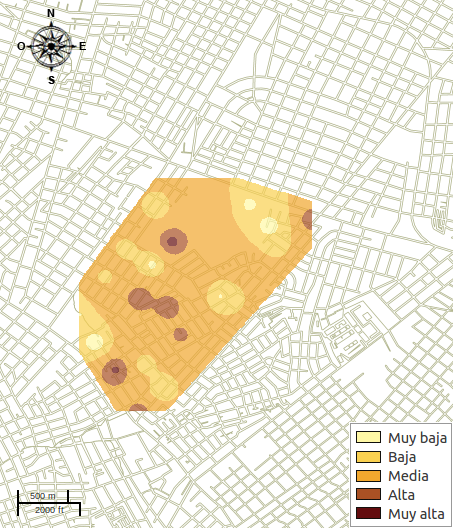
\includegraphics[width=\textwidth]{capitulo-6/graphics/raster/temp-24-0.png}
            \caption{\label{fig:niveles-infestacion-24-a}Primer día de simulación.}
    \end{subfigure}
    ~~
    \begin{subfigure}[b]{0.45\textwidth}
            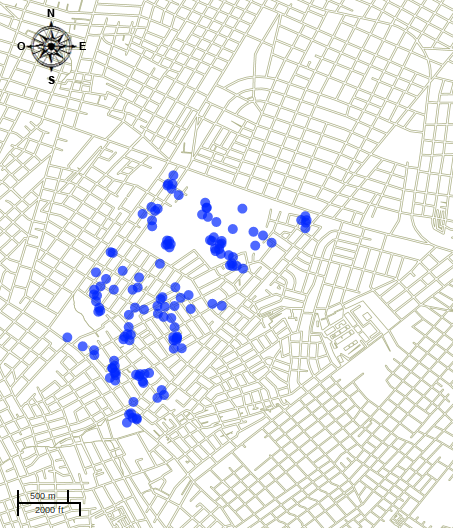
\includegraphics[width=\textwidth]{capitulo-6/graphics/raster/temp-24-16.png}
            \caption{\label{fig:niveles-infestacion-24-b}Día número 17 de simulación.}
    \end{subfigure}

    \begin{subfigure}[b]{0.45\textwidth}
            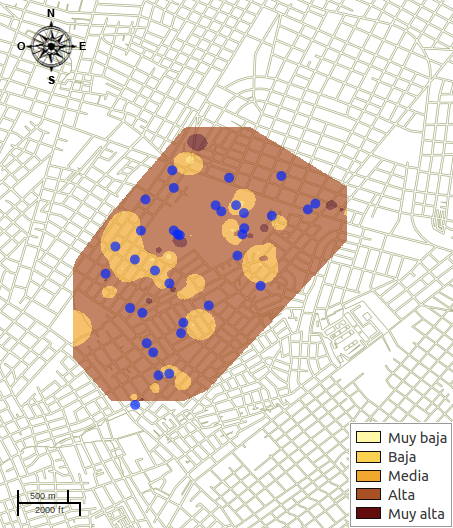
\includegraphics[width=\textwidth]{capitulo-6/graphics/raster/temp-24-26.png}
            \caption{\label{fig:niveles-infestacion-24-c}Día número 27 de simulación.}
    \end{subfigure}
    ~~
    \begin{subfigure}[b]{0.45\textwidth}
            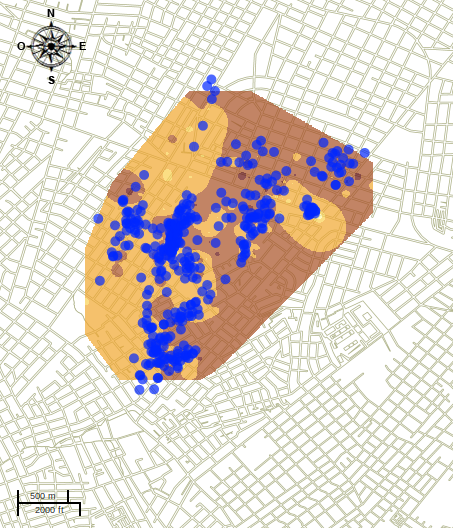
\includegraphics[width=\textwidth]{capitulo-6/graphics/raster/temp-24-49.png}
            \caption{\label{fig:niveles-infestacion-24-d}Día número 50 de simulación.}
    \end{subfigure}

    \caption{\label{fig:niveles-infestacion-24} Mapas de interpolación de la población correspondientes a los días 1, 17, 27 y 50 de simulación a 24 \textcelsius, y la distribución de las hembras adultas (puntos en azul). }
\end{figure}

En la \figref{fig:niveles-infestacion-24-b}, se puede observar que no existen mosquitos en sus
etapas inmaduras, para generar un mapa de interpolación del área, sin embargo se pueden observar la
distribución geográfica de las hembras adultas.

En la \figref{fig:niveles-infestacion-24} se puede observar los niveles de infestación para los
días 1, 17, 27 y 50 del periodo de simulación. En general, se observa el desplazamiento de los
focos de infestación en dirección al noreste, debido a que la dirección del viento utilizada es
igual al sureste y los mosquitos adultos tienden a volar en dirección contraria al viento. Este
desplazamiento se puede observar en las figuras
 \figref{fig:niveles-infestacion-24-a}, \figref{fig:niveles-infestacion-24-c} y
\figref{fig:niveles-infestacion-24-d}.

\subsection{Análisis de la población a 27\textcelsius}
%Población a 27 C
En la \figref{fig:desarrollo-poblacion-27}, se puede observar el comportamiento de la población a
27 \textcelsius, en donde la población de individuos en sus etapas inmaduras va decreciendo hasta
alcanzar un total de 8 individuos en etapas inmaduras en el día 13. A partir del día 10, en la
\figref{fig:desarrollo-poblacion-27}, pueden observarse los primeros mosquitos adultos, donde a
partir del día 14 las hembras adultas, comienzan oviponer, generando un crecimiento de la
población de mosquitos, alcanzando 2 picos importantes en día 24 y 50.

\begin{figure}[!htbp]
    \centering
    \begin{subfigure}[b]{0.45\textwidth}
            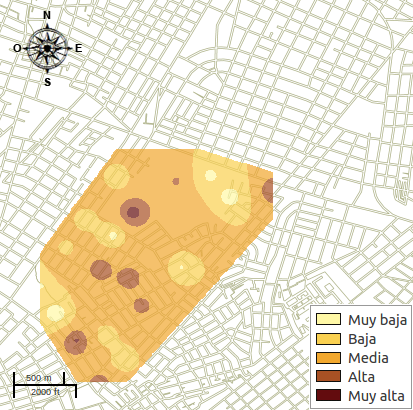
\includegraphics[width=\textwidth]{capitulo-6/graphics/raster/temp-27-0.png}
            \caption{\label{fig:niveles-infestacion-27-a}Primer día de simulación.}
    \end{subfigure}
    ~~
    \begin{subfigure}[b]{0.45\textwidth}
            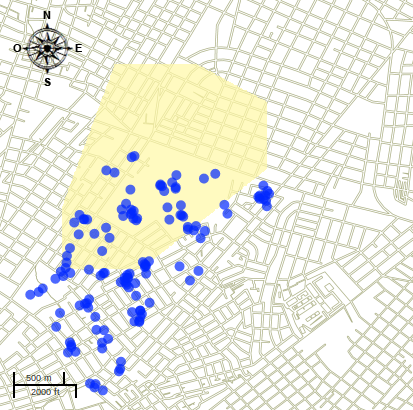
\includegraphics[width=\textwidth]{capitulo-6/graphics/raster/temp-27-12.png}
            \caption{\label{fig:niveles-infestacion-27-b}Día número 13 de simulación.}
    \end{subfigure}

    \begin{subfigure}[b]{0.45\textwidth}
            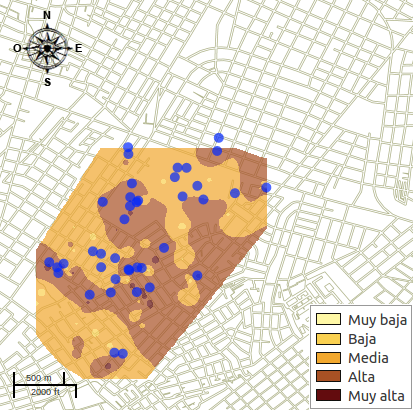
\includegraphics[width=\textwidth]{capitulo-6/graphics/raster/temp-27-22.png}
            \caption{\label{fig:niveles-infestacion-27-c}Día número 23 de simulación.}
    \end{subfigure}
    ~~
    \begin{subfigure}[b]{0.45\textwidth}
            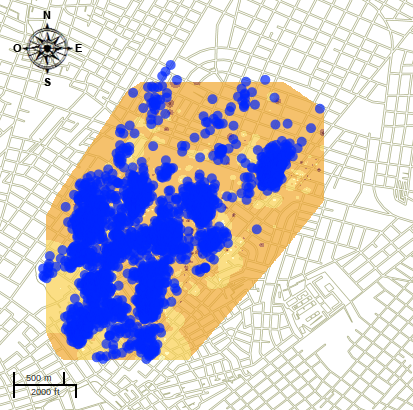
\includegraphics[width=\textwidth]{capitulo-6/graphics/raster/temp-27-49.png}
            \caption{\label{fig:niveles-infestacion-27-d}Día número 50 de simulación.}
    \end{subfigure}

    \caption{\label{fig:niveles-infestacion-27} Mapas de interpolación de la población correspondientes a los días 1, 13, 23 y 50 de simulación a 27 \textcelsius, y la distribución de las hembras adultas (puntos en azul). }
\end{figure}

En la \figref{fig:niveles-infestacion-27-b}, se puede apreciar un nivel de infestación bajo, sin
embargo se puede observar la distribución geográfica de las hembras adultas, lo que implica que la
disminución de la población de mosquitos en sus etapas inmaduras no solo se encuentra influenciada
por la mortalidad diaria, sino también por la aparición de mosquitos adultos producto de la culminación de el ciclo de desarrollo de los mosquitos en etapas inmaduras.

En la \figref{fig:niveles-infestacion-27} se puede observar los niveles de infestación
para los días 1, 12, 22 y 50 del periodo de simulación. En general, se observa el
desplazamiento de los focos de infestación en dirección al noreste, debido a que la dirección del
viento utilizada es igual al sureste y los mosquitos adultos tienden a volar en dirección
contraria al viento. Este desplazamiento se puede observar en las figuras
\figref{fig:niveles-infestacion-27-a},\figref{fig:niveles-infestacion-27-b},
\figref{fig:niveles-infestacion-27-c} y \figref{fig:niveles-infestacion-27-d}.

\subsection{Análisis de la población a 30\textcelsius}
%Población a 30 C
En la \figref{fig:desarrollo-poblacion-30}, se puede observar el comportamiento de la población a
30 \textcelsius, en donde la población de individuos en sus etapas inmaduras va decreciendo hasta
alcanzar un total de 39 individuos en etapas inmaduras en el día 10. A partir del día 8, en la
\figref{fig:desarrollo-poblacion-30}, pueden observarse los primeros mosquitos adultos, donde a
partir del día 11 las hembras adultas, comienzan oviponer, generando un crecimiento de la
población de mosquitos, alcanzando 2 picos importantes en día 21 y 50.

\begin{figure}[!htbp]
    \centering
    \begin{subfigure}[b]{0.45\textwidth}
            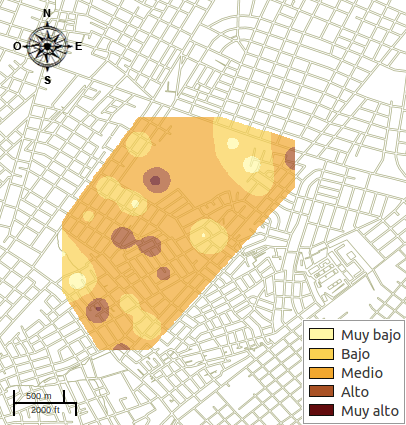
\includegraphics[width=\textwidth]{capitulo-6/graphics/raster/temp-30-0.png}
            \caption{\label{fig:niveles-infestacion-30-a}Primer día de simulación.}
    \end{subfigure}
    ~~
    \begin{subfigure}[b]{0.45\textwidth}
            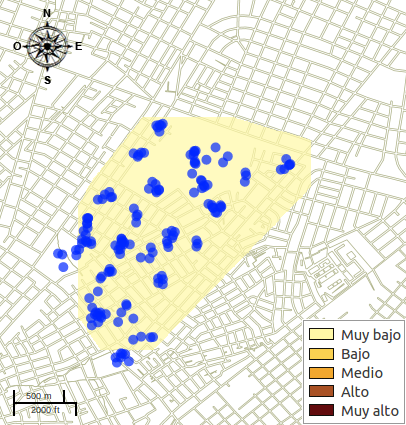
\includegraphics[width=\textwidth]{capitulo-6/graphics/raster/temp-30-9.png}
            \caption{\label{fig:niveles-infestacion-30-b}Día número 10 de simulación.}
    \end{subfigure}

    \begin{subfigure}[b]{0.45\textwidth}
            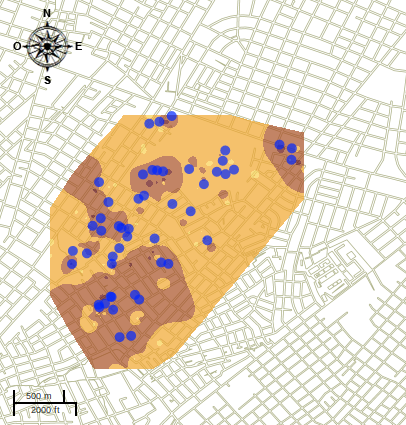
\includegraphics[width=\textwidth]{capitulo-6/graphics/raster/temp-30-20.png}
            \caption{\label{fig:niveles-infestacion-30-c}Día número 21 de simulación.}
    \end{subfigure}
    ~~
    \begin{subfigure}[b]{0.45\textwidth}
            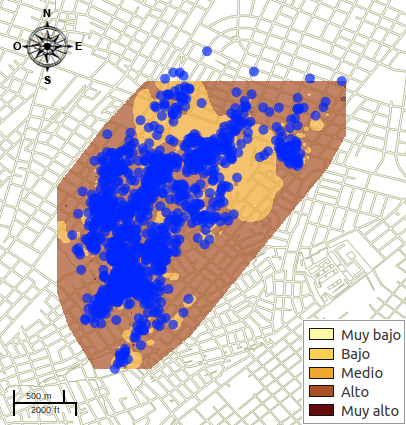
\includegraphics[width=\textwidth]{capitulo-6/graphics/raster/temp-30-35.png}
            \caption{\label{fig:niveles-infestacion-30-d}Día número 50 de simulación.}
    \end{subfigure}

    \caption{\label{fig:niveles-infestacion-30} Mapas de interpolación de la población correspondientes a los días 1, 10, 21 y 35 de simulación a 30 \textcelsius, y la distribución de las hembras adultas (puntos en azul). }
\end{figure}

En la \figref{fig:niveles-infestacion-30-b}, se puede apreciar un nivel de infestación bajo, sin
embargo se puede observar la distribución geográfica de las hembras adultas, lo que implica que la
disminución de la población de mosquitos en sus etapas inmaduras no solo se encuentra influenciada
por la mortalidad diaria, sino también por la aparición de mosquitos adultos producto de la culminación de el ciclo de desarrollo de los mosquitos en etapas inmaduras.

En la \figref{fig:niveles-infestacion-30} se puede apreciar los niveles de infestación
para los días 1, 10, 21 y 35 del periodo de simulación. En general, se observa el
desplazamiento de los focos de infestación en dirección al noreste, debido a que la dirección del
viento utilizada es igual al sureste y los mosquitos adultos tienden a volar en dirección
contraria al viento. Este desplazamiento se puede observar en las figuras
\figref{fig:niveles-infestacion-30-a},\figref{fig:niveles-infestacion-30-b},
\figref{fig:niveles-infestacion-30-c} y \figref{fig:niveles-infestacion-30-d}.

\subsection{Análisis de la población a 34\textcelsius}
%Población a 34 C
En la \figref{fig:desarrollo-poblacion-34}, se puede observar el comportamiento de la población a
34 \textcelsius, en donde la población de individuos en sus etapas inmaduras va decreciendo hasta
alcanzar un total de 49 individuos en etapas inmaduras en el día 11. A partir del día 9, en la
\figref{fig:desarrollo-poblacion-34}, pueden observarse los primeros mosquitos adultos, donde a
partir del día 12 las hembras adultas, comienzan oviponer, generando un crecimiento de la
población de mosquitos, alcanzando 2 picos importantes en día 21 y 50.

\begin{figure}[!htbp]
    \centering
    \begin{subfigure}[b]{0.45\textwidth}
            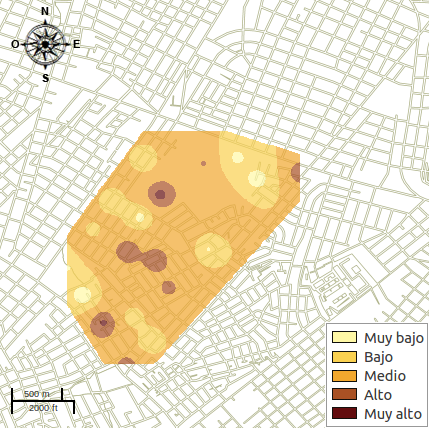
\includegraphics[width=\textwidth]{capitulo-6/graphics/raster/temp-34-0.png}
            \caption{\label{fig:niveles-infestacion-34-a}Primer día de simulación.}
    \end{subfigure}
    ~~
    \begin{subfigure}[b]{0.45\textwidth}
            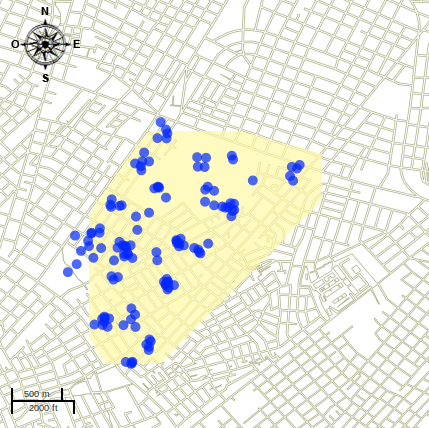
\includegraphics[width=\textwidth]{capitulo-6/graphics/raster/temp-34-10.png}
            \caption{\label{fig:niveles-infestacion-34-b}Día número 11 de simulación.}
    \end{subfigure}

    \begin{subfigure}[b]{0.45\textwidth}
            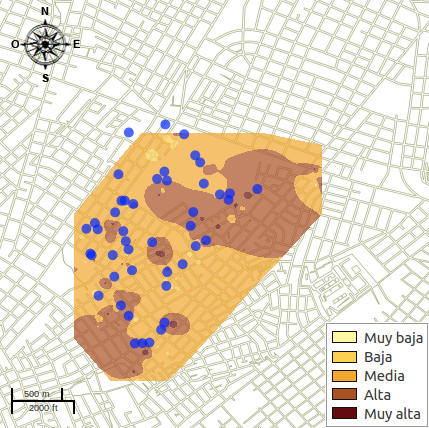
\includegraphics[width=\textwidth]{capitulo-6/graphics/raster/temp-34-20.png}
            \caption{\label{fig:niveles-infestacion-34-c}Día número 21 de simulación.}
    \end{subfigure}
    ~~
    \begin{subfigure}[b]{0.45\textwidth}
            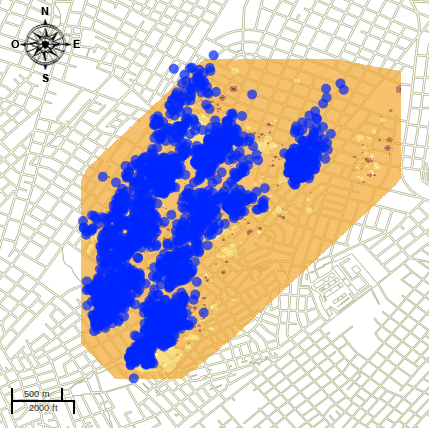
\includegraphics[width=\textwidth]{capitulo-6/graphics/raster/temp-34-42.png}
            \caption{\label{fig:niveles-infestacion-34-d}Día número 43 de simulación.}
    \end{subfigure}

    \caption{\label{fig:niveles-infestacion-34} Mapas de interpolación de la población correspondientes a los días 1, 11, 21 y 43 de simulación a 34 \textcelsius, y la distribución de las hembras adultas (puntos en azul). }
\end{figure}

En la \figref{fig:niveles-infestacion-34-b}, se puede apreciar un nivel de infestación bajo, sin
embargo se puede observar la distribución geográfica de las hembras adultas, lo que implica que la
disminución de la población de mosquitos en sus etapas inmaduras no solo se encuentra influenciada
por la mortalidad diaria, sino también por la aparición de mosquitos adultos producto de la
culminación de el ciclo de desarrollo de los mosquitos en etapas inmaduras.

En la \figref{fig:niveles-infestacion-34} se puede apreciar los niveles de infestación
para los días 1, 11, 21 y 43  del periodo de simulación. En general, se observa el
desplazamiento de los focos de infestación en dirección al noreste, debido a que la dirección del
viento utilizada es igual al sureste y los mosquitos adultos tienden a volar en dirección
contraria al viento. Este desplazamiento se puede observar en las figuras
\figref{fig:niveles-infestacion-34-a},\figref{fig:niveles-infestacion-34-b},
\figref{fig:niveles-infestacion-34-c} y \figref{fig:niveles-infestacion-34-d}.

